\section{Rolling Road PSoC} \fxnote{burde vel bare hedde Rolling Road... da det hele tiden bliver beskrevet som Rolling Road --- LB }
The Rolling Road's function is to test a subjects efficiency, at a specified torque or force. To do so it has to measure both the mechanic and electric power usage and calculate the efficiency based on those numbers.\\

\fxnote{Omformuler - JH}
It has to be easy to use from a control unit \vref{Rolling_Road_GUI} through a serial COM connection. The control unit can send a list of commands, to change PID parameter, change wanted torque and calibrate sensors. The Rolling road will also feedback information from all sensors, and calculation of power and efficiency.\\
\subsection{Design}
The rolling road is made in c but is written in a more object form to look like c++\fxnote{Arrrrghh, det går vidst ikke - JH}. Because it is easier to design it as a objective program. To design the solution, a class diagram was made see Rolling road doc\fxnote{lav reference}.\\

The design of Rolling Road consist of three things: regulating, measure and communication. Where all these work together.\\

The reason that it is programmed in c and not c++ are because PSoC creator don't have a built-in c++ compiler\fxnote{Ikke nødvendigt at beskrive - JH}. 
\subsection{Implementation}
In the implementation another problem was made clear, the measurements of sensors and the calculation were very time critical. To get a better overview over the flow, a flow-diagram was made see \vref{fig:data_flow_diagram}.\\

\fxnote{Omformuler indtil moving average filter - JH}
This flow-diagram was used to design the flow of data, and there the calculation should happen. As seen in the diagram the regulator gets the value faster then the control unit. Because to big time delay would made the system unstable.\\

The different signals from the sensors goes though a couple of steps before they are calculated and passed on. To save as much CPU time as possible, DMA\fxnote{Was? - JH} was setup to make the flow use less CPU time. This is done on the torque sensor. Because it has be measured with as little time delay as possible. Where are implemented some decimation filter in the design, because the sensor are measured with a big sample frequency around 50 kSample/s. Where the PID regulator only runs with 2 kSample/s and the data transmitting to the control unit only run with a speed of 2-100 Sample/s.\\
There is also implemented a small exponential moving average filter, that smooths all data before sending to the control unit.    
\begin{figure}[H]
	\centering
	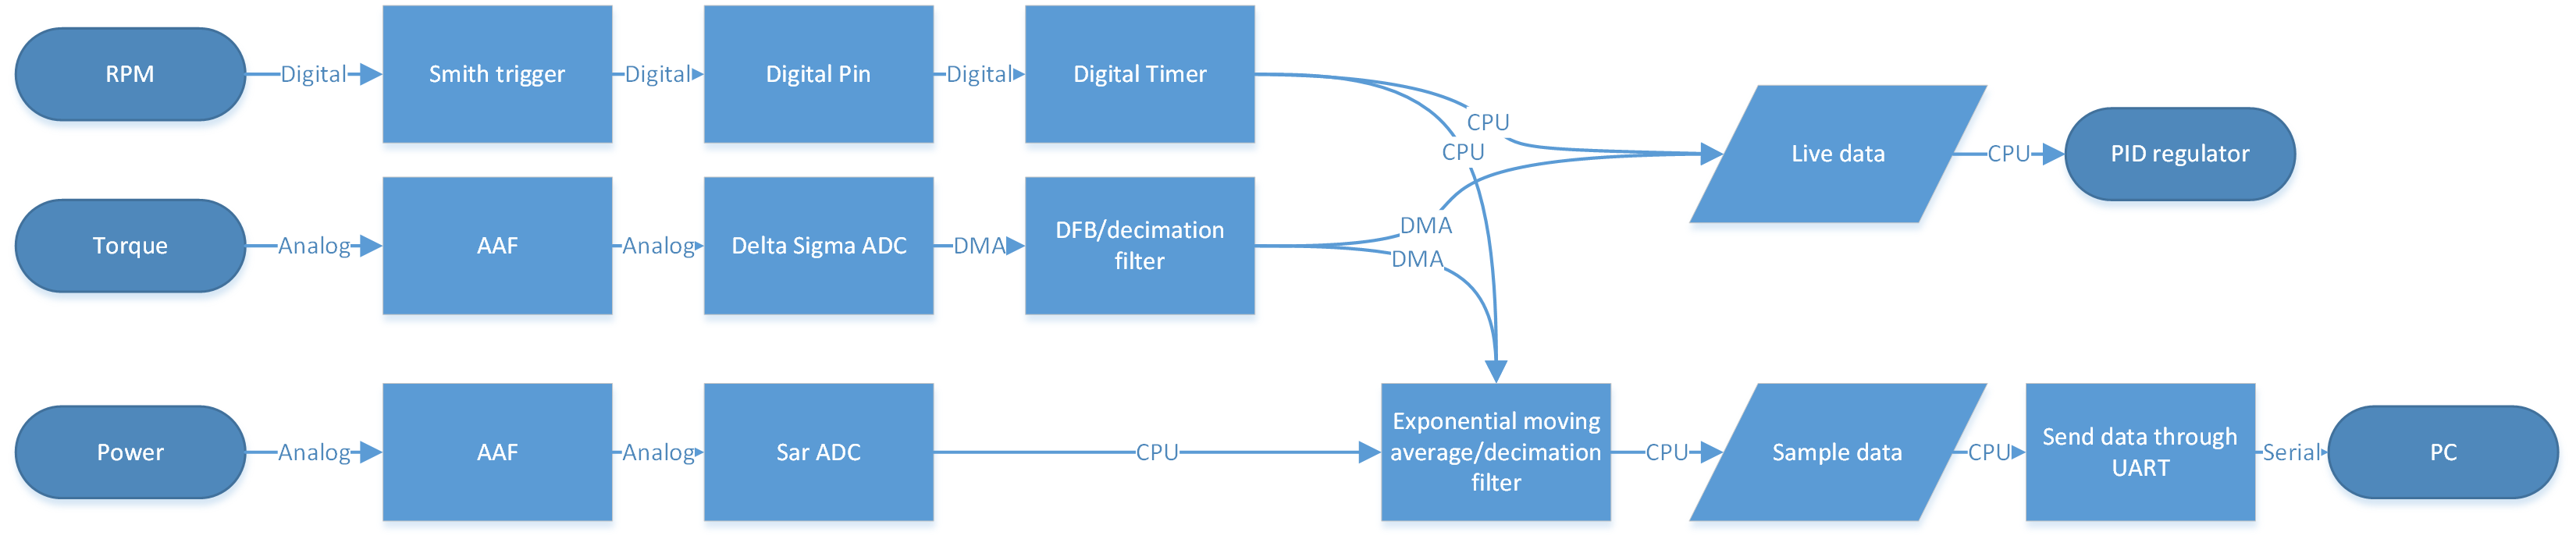
\includegraphics [width=6in]{../Documentation_RR/Software/Pictures/data-flow.png}
	\caption{Rolling Road data-flow diagram.}
	\label{fig:data_flow_diagram}
\end{figure}
\subsection{Test}
To test Rolling Road a test stand was setup with a test car figure \ref{fig:RR_first_test}. Where the measure of the car was made. \fxnote{Få lige fat i det originale billede, opløsningen er dårlig og laimonas navn står oppe i venste hjørne - JH} 
\begin{figure}[H]
	\centering
	\includegraphics [width=3in]{SubPages/Images/jens_test.png}
	\caption{First test of the old AU car.}
	\label{fig:RR_first_test}
\end{figure}
After a half hour test a efficiency diagram could be made from the data \ref{fig:RR_first_test_result}.

\begin{figure}[H] 
	\centering
	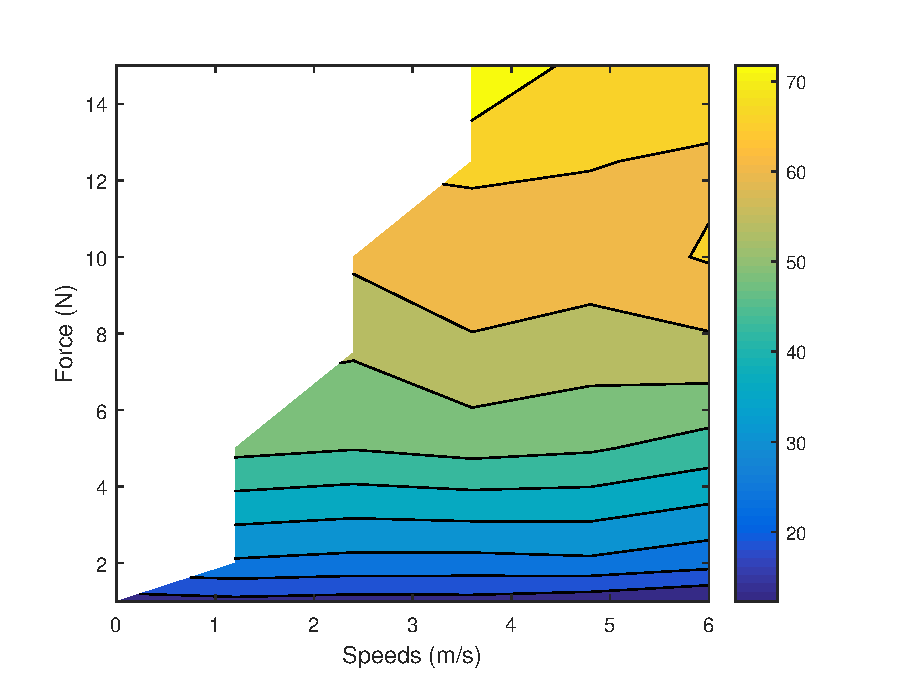
\includegraphics [width=3in]{SubPages/Images/RR_test_result.eps}
	\caption{efficiency diagram of the first test, the value is in \% efficiency.}
	\label{fig:RR_first_test_result}
\end{figure}
This result is not close enough to the efficiency what was calculated by a mechanical-engineer. But the car is not in the best shape, and it was not fastened to the Rolling Road. So there is many places there is efficiency lost.


